\section{Object 1}
\markright{Object 1}

\begin{figure}[H]
  \centering

  \begin{subfigure}[b]{0.45\textwidth}
    \centering
    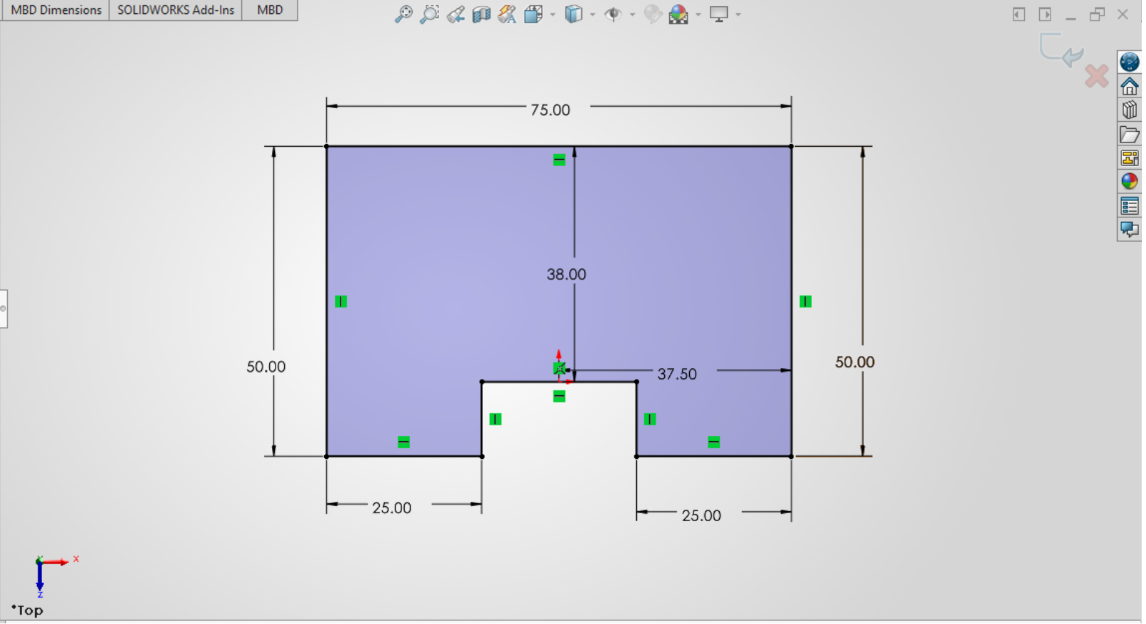
\includegraphics[width=\textwidth, keepaspectratio]{lab-01/assets/object-1/object-1-snap-1.png}
  \end{subfigure}
  \begin{subfigure}[b]{0.45\textwidth}
    \centering
    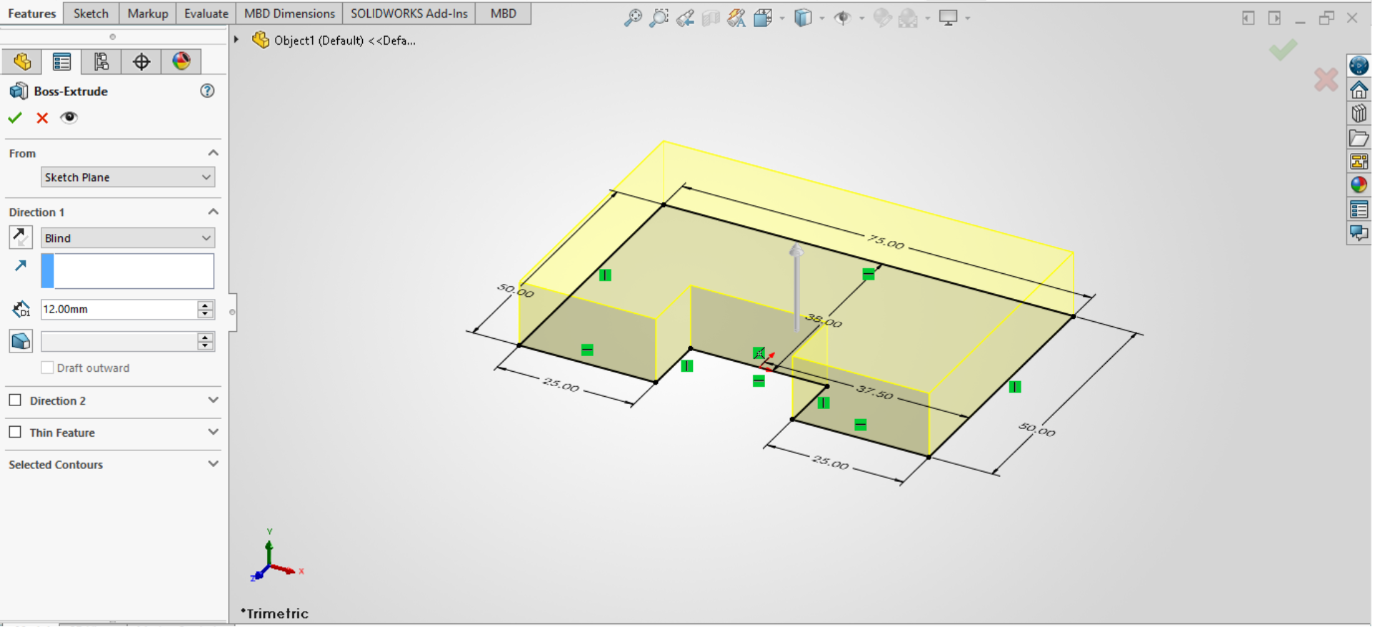
\includegraphics[width=\textwidth, keepaspectratio]{lab-01/assets/object-1/object-1-snap-2.png}
  \end{subfigure}
  \begin{subfigure}[b]{0.90\textwidth}
    \centering
    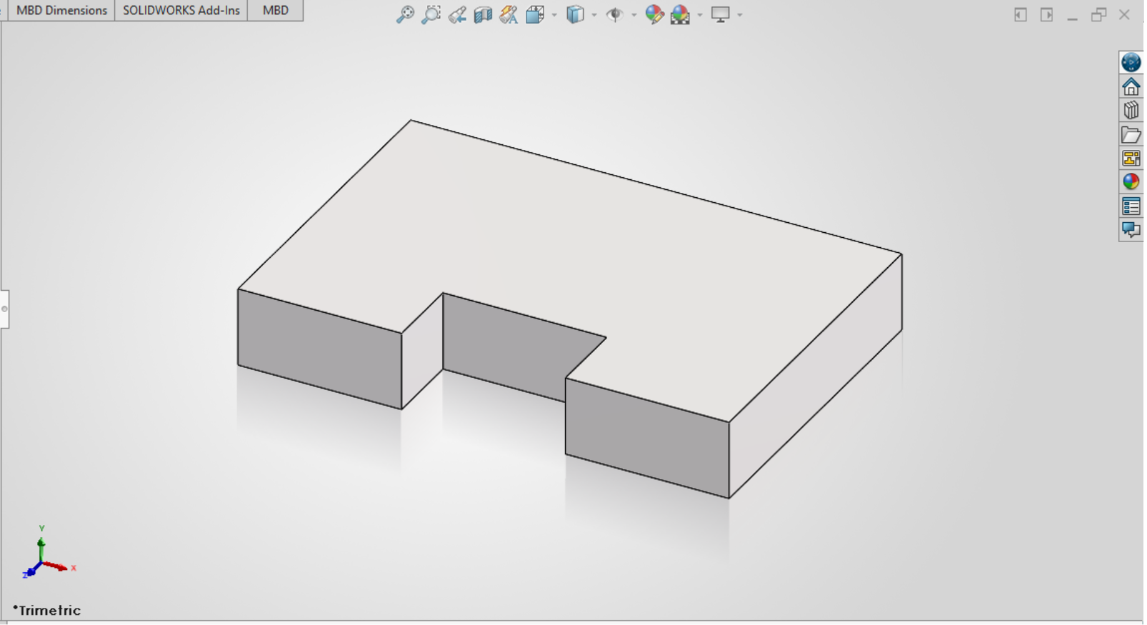
\includegraphics[width=\textwidth, keepaspectratio]{lab-01/assets/object-1/object-1-snap-3.png}
  \end{subfigure}
  \begin{subfigure}[b]{0.45\textwidth}
    \centering
    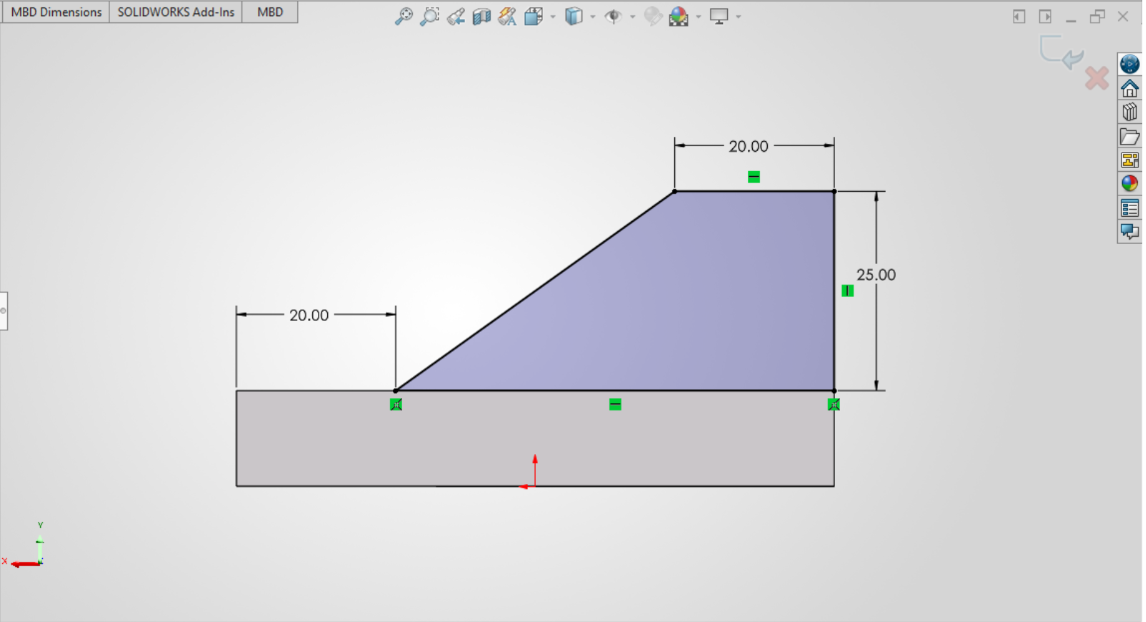
\includegraphics[width=\textwidth, keepaspectratio]{lab-01/assets/object-1/object-1-snap-4.png}
  \end{subfigure}
  \begin{subfigure}[b]{0.45\textwidth}
    \centering
    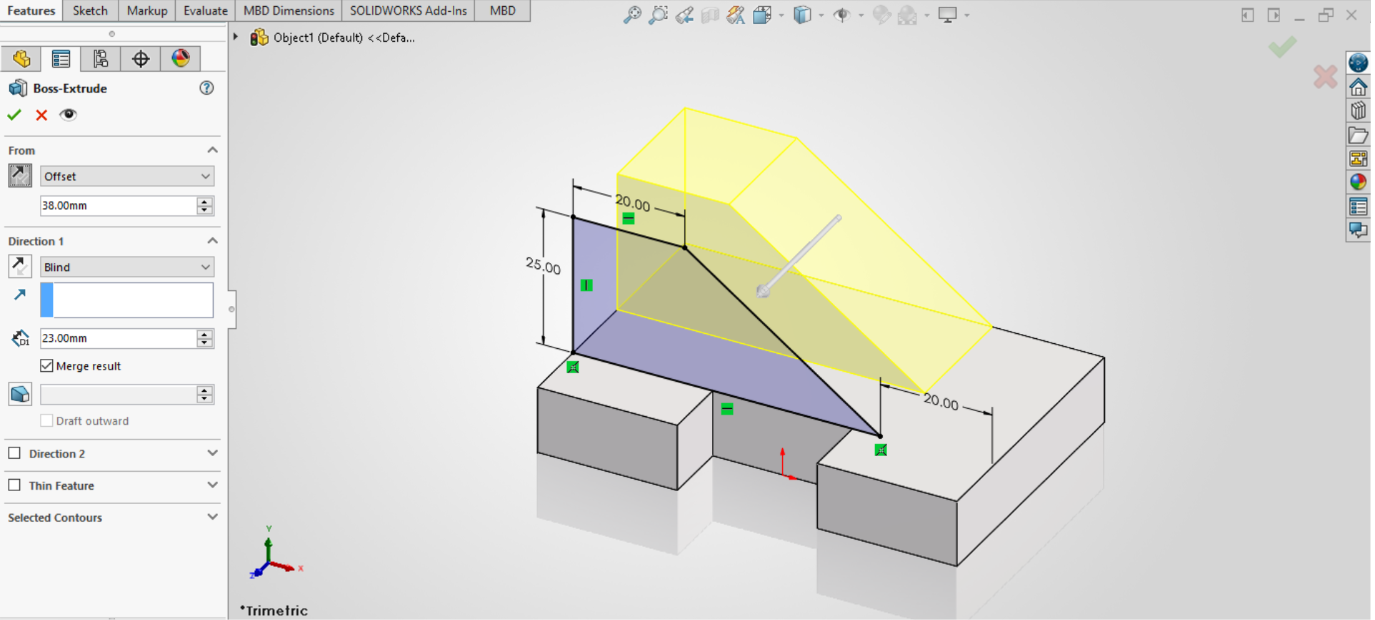
\includegraphics[width=\textwidth, keepaspectratio]{lab-01/assets/object-1/object-1-snap-5.png}
  \end{subfigure}
  \begin{subfigure}[b]{0.90\textwidth}
    \centering
    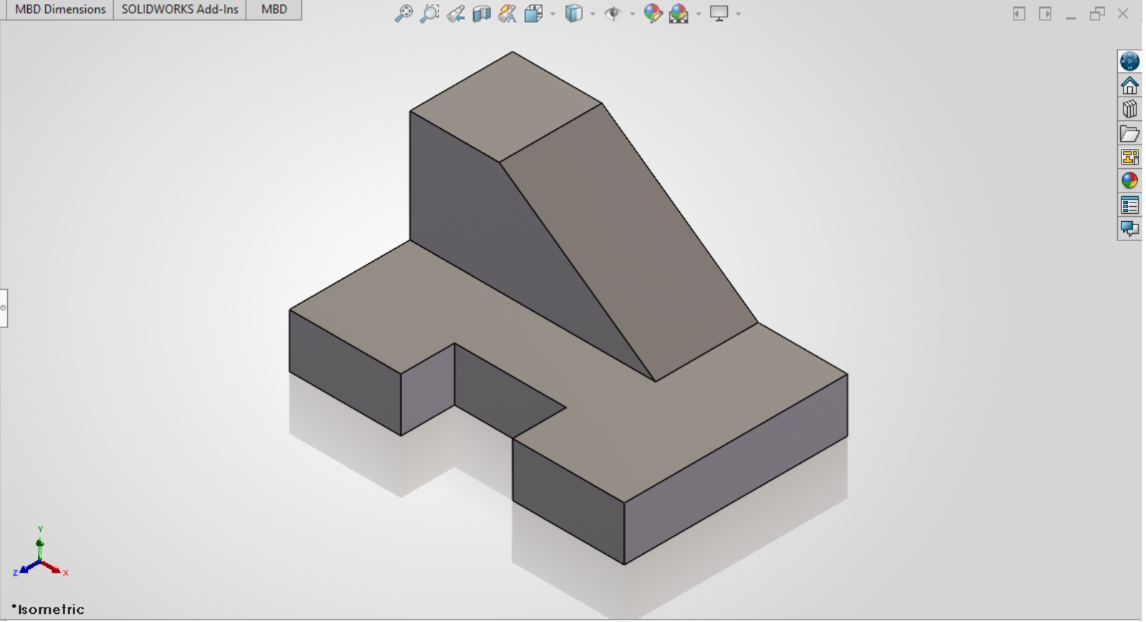
\includegraphics[width=\textwidth, keepaspectratio]{lab-01/assets/object-1/object-1-snap-6.png}
  \end{subfigure}

  \caption{Snapshots while Designing Object 1 in Solidworks}
  \label{lab01_object_1}
\end{figure}

